\section{MF Tokens and Lemmas \label{sec:tokens_lemmas}}

This section aim to evaluate the vector representation using the most frequent (MF) tokens and lemmas.

\subsection{MF Tokens and Lemmas Method}

The MF method only have one parameter: $n$.
$n$ is the number of most frequent items.
For the tokens and lemmas text representation, no clear $n$ value is to choose over others.
Depending on the documents' length, previous studies have shown that using $n$ value between $50$ and $500$ tends to produce good results for the token text representation~\cite{savoy_text_representation}.

One of the main advantage of this representation is that they can be easily explained.
The feature vectors can be show to the user.
It represents the proportion of the most frequent words in a document.
If $n$ is too large to present to the user, a dimensionality reduction with, for example, the principal component analysis (PCA) can be helpful~\cite{savoy_stylo}.

Instead of using directly the words to create the feature vector, another possibility is to use the lemma corresponding to each word, e.g. the sentence \textit{i saw two men with a saw} its lemmatized version is : \textit{i see two man with a saw}.
This requires advanced text preprocessing, but it can remove ambiguity.

The 40 most frequent tokens and lemmas for the St-Jean corpus are showed in Table~\ref{tab:tokens_occurences_st_jean} and Table~\ref{tab:lemmas_occurences_st_jean} in annex.

\subsection{MF Tokens and Lemmas evaluation \label{sec:tokens_lemmas_eval}}

Here, the goal is to compare two similar text representations, which are the token representation and the lemmatize representation.
Rank list using these representations are created and evaluated.
The corpus used for this experiment is St-Jean, since have the two text representation and is a large corpus.

The proposed methodology is to create rank lists for every proposed distance measures (ref. Section~\ref{sec:vectors_distances}) on the two text representations.
The $n$ value is also explored between 250 and 2000 with a step of 250.

The two plots in Figure~\ref{fig:tokens_lemmas} show the average precision (AP) for the resulting rank lists over $n$ for each distance measure.
Table~\ref{tab:tokens_lemmas} in annex show the values used to create this graph.

This representation seem to have good results with $n=500$ for most of the distance metrics, this corroborates previous studies results.

Few distance metrics, such as Manhattan distance, Tanimoto distance or Clark distance can give better results with slightly bigger vectors (750 or 1000 MF tokens/lemma).
For most distance metrics, the token representation provide on both corpora a greater average precision compared to the lemma representation.

An interesting example to be worth noticing concern the Manhattan distance.
The AP when using the token representation tends to decrease faster than the AP for the lemma representation as $n$ increase.

The Euclidean distance seems to be the least appropriate distance measure for this task.
The Clark distance have a really poor average precision when the MF tokens vector is too small, but after reaching 500 it produces one of the best pay-off of the experiment.

Using the best $n$ with these text representations, the best distance metric can increase the average precision by a factor of $13$ to $17$ \%.
Over all, the Cosine distance seem to be one of the most appropriate choice when dealing with these corpora and text representations.

The retained distance metrics and $n$-MF for the tokens text representations are:
\begin{itemize}
  \item 750-MF tokens with Cosine distance.
  \item 750-MF tokens with Clark
  \item 750-MF tokens with Manhattan
  \item 750-MF tokens with Tanimoto
\end{itemize}

The $n = 750$ is used for every distance metric, since the results between $500$ and $1000$ are similar for most distance metrics.

Even though, the lemma representation sometimes give betters than the tokens one.
Only the tokens' representation is kept since it is obtainable more easily and no significant improvements are observed.

\begin{figure}
  \centering
  \caption{Tokens and Lemmas representation over number of MF tokens using different distances metrics}
  \label{fig:tokens_lemmas}

  \subcaption{Tokens}
  \label{fig:tokens}
  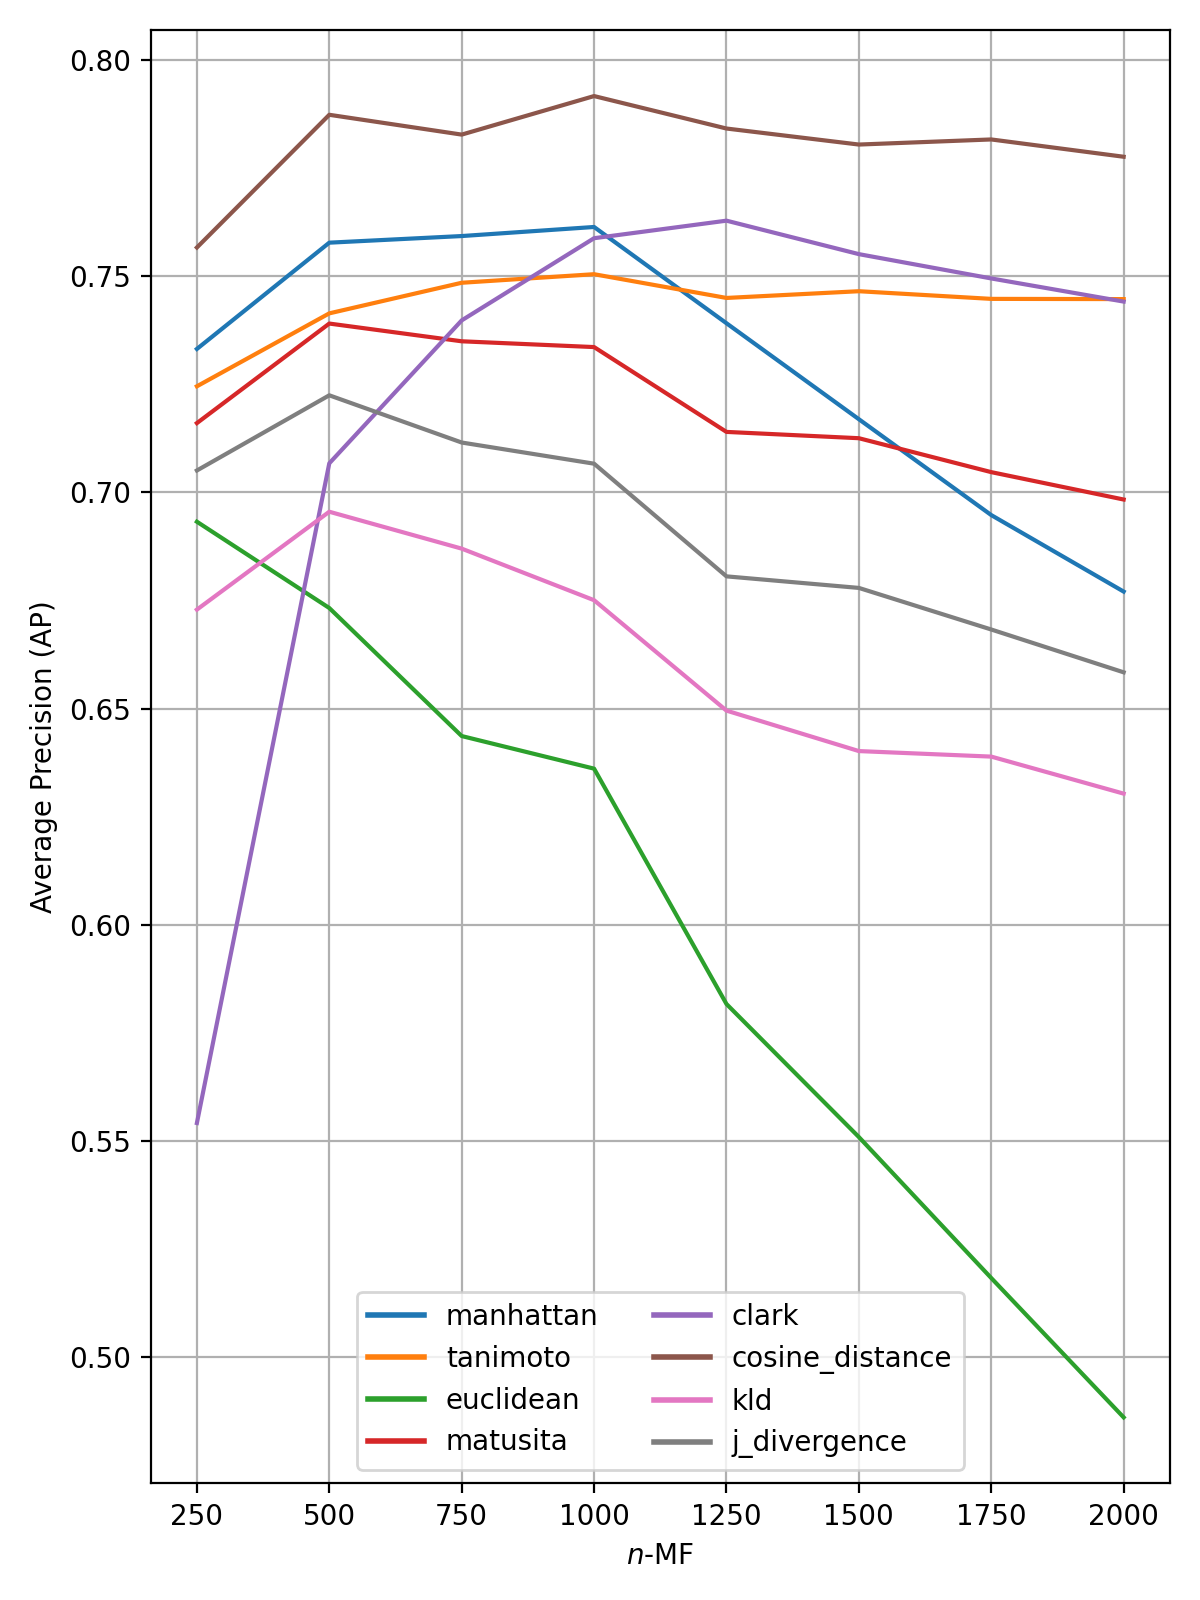
\includegraphics[width=0.9\linewidth]{img/mf_tokens.png}

  \vspace{0.5cm}

  \subcaption{Lemmas}
  \label{fig:lemmas}
  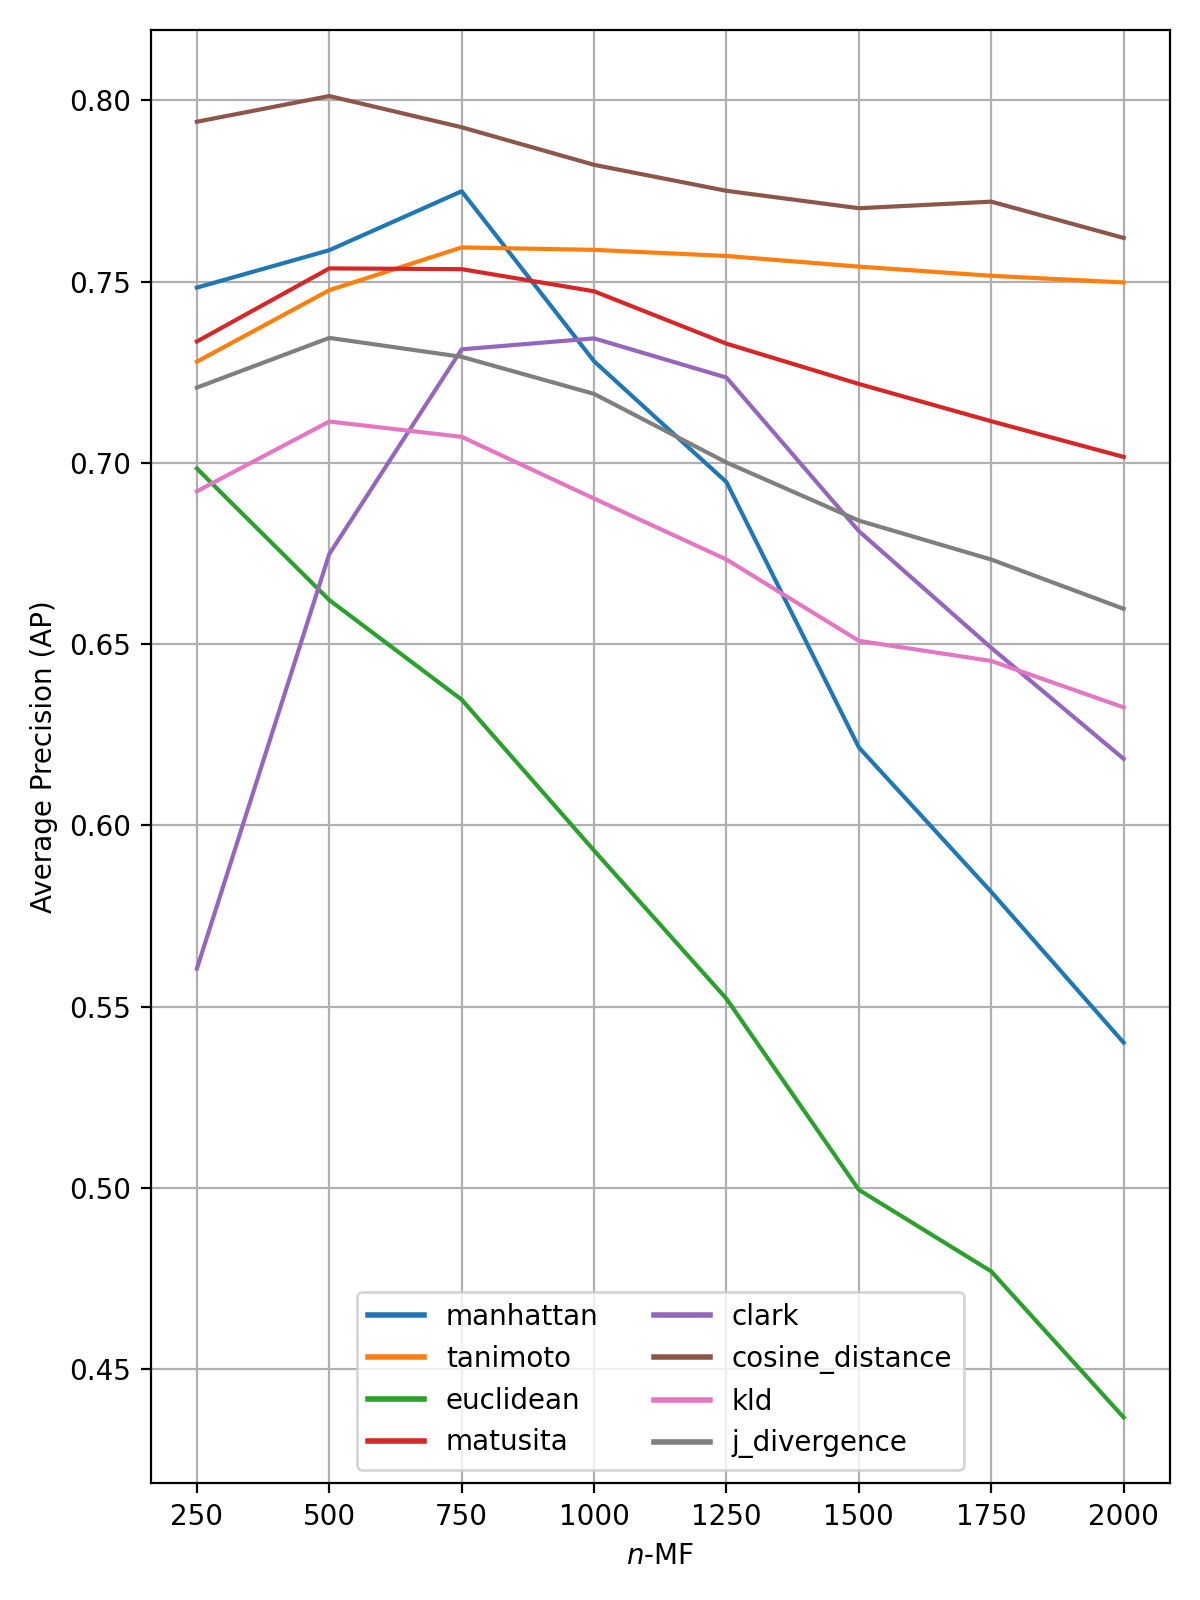
\includegraphics[width=0.9\linewidth]{img/mf_lemmas.png}
\end{figure}

\subsection{Text Size\label{sec:importance_of_text_size}}

For this study, an experiment on the St-Jean corpus is accomplished, to show the importance of having large documents.
To test this, the number of token is artificially modified by considering only the $t$ first tokens of each text.
Here $t$ range between 9000 and 250 with steps of 250 tokens.
From these texts, the $750$-MF tokens text representation is used in conjunction with the Z-Score normalized Cosine distance to compute the rank lists.

Figure~\ref{fig:degradation} show the rank lists evaluated using the average precision, RPrec and HPrec over the number of tokens.
The full evaluation is showed in Table~\ref{tab:degradation} in annex.

Every metric decrease over the text size.
This indicates that it becomes harder to determinate documents pairs with the same author as the text size decrease.

PAN16 corpus is a difficult corpus due to its small size, thus extracting reliable features for each text to estimate each style is also a difficult task.
After multiple tests, the PAN @ CLEF 2016 corpus is not used further in this study due to its difficulty in finding reliable Stylometric clues.
For this study, having standard and easier corpus is required in order to show the proposed methods.

\begin{figure}
  \centering
  \caption{St-Jean ranks list evaluation on AP, RPrec and HPrec over the text size. Rank list computed using $750$-MF tokens and the Z-Score normalized Cosine distance}
  \label{fig:degradation}
  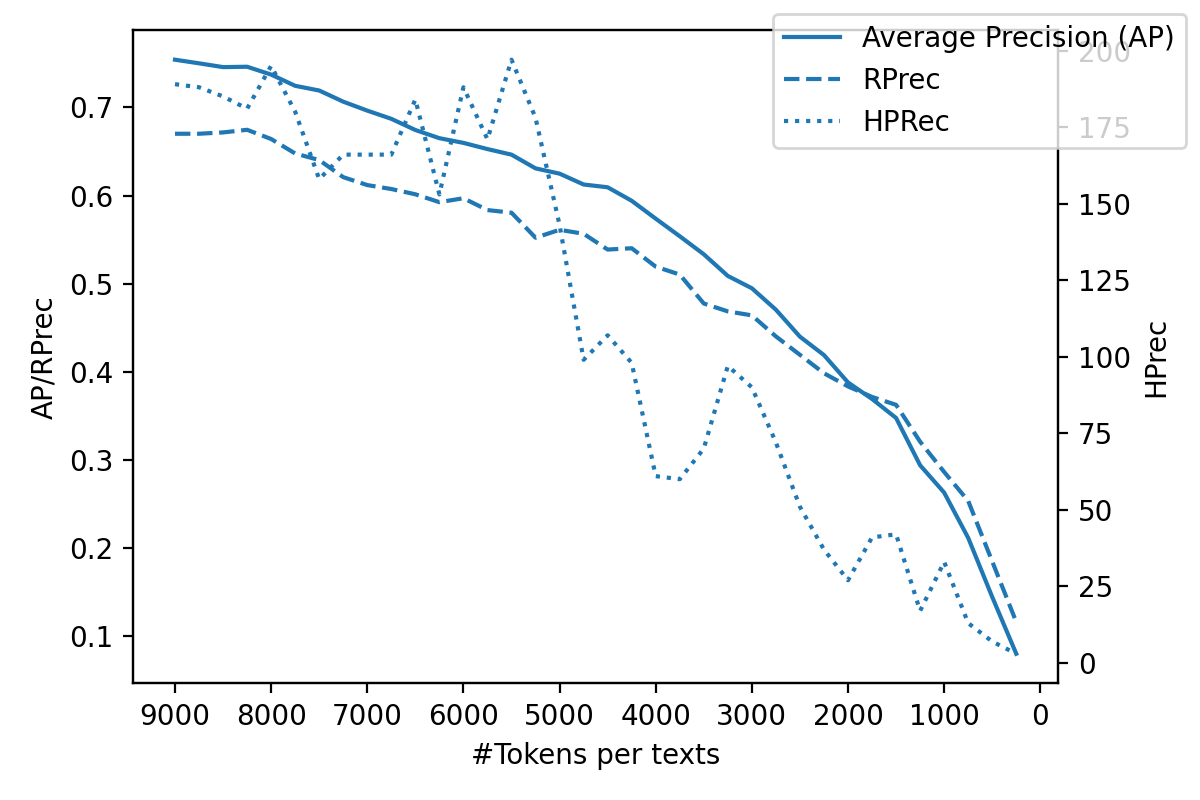
\includegraphics[width=\linewidth]{img/degradation.png}
\end{figure}

\subsection{Most Frequent Items Restriction \label{sec:influance_mf_restriction}}

Previously, the MF method was proposed to limit the items used to only the most frequents in the vocabulary of a corpus.
This experiment aim to show the importance of limiting the items used when creating the vector representing the document.

Three approach are compared:
\begin{enumerate}
  \item
  \textit{every token} : Use the whole corpus vocabulary to create the feature vector.
  \item
  \textit{without hapax legomena} : Every token appearing more than once are used to create these vectors.
  \item
  \textit{750-MF} : The vector represents the 750 most frequent tokens.
\end{enumerate}

The eight proposed distance measures are evaluated for the three approach using the average precision metric on the three literature corpora.
To understand more easily the results for the three approach, the \textit{every token} approach is used as a baseline, from where the average precision gain is computed.

Table~\ref{tab:baseline_every_token} show the average precision baseline using the \textit{every token} approach.
Table~\ref{tab:gain_without_hapax_legomena} and Table~\ref{tab:gain_750_mf} show the gain over the baseline for the \textit{without hapax legomena} approach and \textit{750-MF} approach respectively.

When looking at the baseline : the Manhattan, Euclidean and Clark distance measure have a poor average precision, all are below 0.3 in average.
The other metric have medium to good results.
It ranges from 0.58 for the KLD to 0.79 with the Cosine distance.
The Cosine distance with \textit{every token} reach a 0.91 average precision for the Oxquarry corpus.
When removing hapax legomena, for most distance metrics the gain in average precision is limited, except for the Clark distance where the mean average precision rise from 0.3 to 0.5.
After limiting to the 750-MF, the Manhattan, Euclidean and Clark distance, the ones that had poor results for the baseline increase their average precision by around 48\% which correspond to an average precision of 0.71, 0.63 and 0.78 respectively, which makes them in the same range as the other metrics in the baseline.
Across every metric and corpus, removing hapax legomena increase the average precision in average by 0.04, and limiting to the $750$-MF by 0.21.
This clearly indicate the importance of limiting the size of the vector for most distance metrics.

From this experiment, each distance metric can be placed in one of the two following categories : the ones sensible to large and noisy vectors, the ones not sensible.
In the first category are : Manhattan, Clark and Euclidean, in the second : Cosine, Matusita and Tanimoto.
As for KLD and JD, they are nor in the first nor the second, since both of them had a small gain in regard to the Oxquarry corpus but larger gain for the St-Jean corpus.
Further, test are required to classify these distance metrics.

\begin{table}
  \centering
  \caption{Rank lists average precision depending on the number of token used}

  \subcaption{Baseline: \textit{every token}}
  \label{tab:baseline_every_token}
  \resizebox{\linewidth}{!}{
  \begin{tabular}{l r r r|r}
    \toprule
    Distance & Oxquarry & Brunet & St-Jean & Mean \\
    \midrule
    Manhattan & 0.27 & 0.21 & 0.17 & 0.22 \\
    Tanimoto  & 0.63 & 0.65 & 0.70 & 0.66 \\
    Euclidean & 0.19 & 0.19 & 0.08 & 0.15 \\
    Matusita  & 0.61 & 0.63 & 0.62 & 0.62 \\
    Clark     & 0.40 & 0.28 & 0.21 & 0.30 \\
    Cosine    & 0.91 & 0.73 & 0.73 & 0.79 \\
    KLD       & 0.58 & 0.59 & 0.56 & 0.58 \\
    JD        & 0.59 & 0.63 & 0.59 & 0.60 \\
    \midrule
    Mean      & 0.52 & 0.49 & 0.46 & 0.49 \\
    \bottomrule
  \end{tabular}
  }

  \vspace{0.5cm}

  \subcaption{Gain \textit{without hapax legomena} over baseline}
  \label{tab:gain_without_hapax_legomena}
  \resizebox{\linewidth}{!}{
  \begin{tabular}{l r r r|r}
    \toprule
    Distance & Oxquarry & Brunet & St-Jean & Mean \\
    \midrule
    Manhattan & +0.10 & +0.05 & +0.02 & +0.06 \\
    Tanimoto  & -0.00 & +0.01 & +0.00 & +0.01 \\
    Euclidean & +0.11 & +0.01 & +0.00 & +0.04 \\
    Matusita  & -0.01 & +0.01 & -0.01 & -0.00 \\
    Clark     & +0.19 & +0.16 & +0.25 & +0.20 \\
    Cosine    &  0.02 & -0.02 & -0.02 & -0.01 \\
    KLD       & -0.02 & +0.02 & -0.01 & -0.00 \\
    JD        & -0.01 & +0.01 & -0.02 & -0.01 \\
    \midrule
    Mean      & +0.05 & +0.03 & +0.03 & +0.04 \\
    \bottomrule
  \end{tabular}
  }

  \vspace{0.5cm}

  \subcaption{Gain \textit{750-MF} over baseline}
  \label{tab:gain_750_mf}
  \resizebox{\linewidth}{!}{
  \begin{tabular}{l r r r|r}
    \toprule
    Distance & Oxquarry & Brunet & St-Jean & Mean \\
    \midrule
    Manhattan & +0.40 & +0.47 & +0.59 & +0.49 \\
    Tanimoto  & +0.00 & +0.03 & +0.05 & +0.03 \\
    Euclidean & +0.43 & +0.45 & +0.57 & +0.48 \\
    Matusita  & +0.02 & +0.05 & +0.12 & +0.06 \\
    Clark     & +0.49 & +0.44 & +0.53 & +0.48 \\
    Cosine    & -0.02 & -0.02 & +0.06 & +0.01 \\
    KLD       & +0.02 & +0.07 & +0.12 & +0.07 \\
    JD        & +0.02 & +0.04 & +0.12 & +0.06 \\
    \midrule
    Mean      & +0.17 & +0.19 & +0.27 & +0.21 \\
    \bottomrule
  \end{tabular}
  }
\end{table}

\subsection{Frequent Errors \label{sec:frequent_errors}}

For this experiment, the goal is to try to understand the errors in the system, in this case the false links (document pairs with different authors) highly ranked on different rank lists.
The rank list quality is high based on the text representation and the distance function, but mostly on the first.
The previous statement can be deduced by the following reasoning : For example when using the $n$-MF method, if two documents feature vector are closely related (nearly identical), no matter the distance function they should have a low distance, since every distance function should give a distance of 0 when computing the distance between two identical vectors.

We believe some errors in the system are due to documents having close feature vectors values even though they are not from the same authors.
To motivate this statement, the following experiment is realized.

The four token-based retained rank list from the St-Jean corpus are used, see Section~\ref{sec:tokens_lemmas_eval}.
These four rank lists share the same text representation, in this case the relative frequency of the $750$-MF tokens as feature vector, only the distance function used to create the rank lists are different.
For the sake of this experiment, we define \textit{frequent errors} as : \textit{Links appearing in the top 20 false links of at least 3 out of the 4 rank lists}.

The goal is to compare the two documents feature vector for special links.
In our case, the links chosen are : Frequent errors, linked ranked first (most similar vectors, according to the distance function), link ranked last (the least similar vectors) and ranked HPrec-th in a rank list.

To perform a comparison, the feature vector is visualized using a bar plot.
The visualization is based on the $750$-MF tokens vector, since the rank lists were created using this vector size.
To be able to understand more easily the visualization, the values have been sorted by the mean relative frequencies and use a logarithmic scale.

When a large proportion of the vectors overlap, it indicates a high similarity between the MF vectors.
Both document style are close when their feature vector are closely related.
Visually when most of the surface overlap, the distance function will give a low value, and with a correct distance measure this link should be ranked high in the rank list.

Figure~\ref{fig:mf_vector_error} show the feature vector of two frequent errors document pairs (\textit{Cinq-Mars}$_{48}$ from Vigny / \textit{Les trois mousquetaires}$_{62}$ from Dumas and \textit{Bel-Ami}$_{10}$ from Maupassant / \textit{Madame Bovary}$_{52}$ from Flaubert), these link appear in the top 20 false links of 3 out 4 rank lists.
The frequent errors vector pairs presented in Figure~\ref{fig:mf_vector_error} can be visually compared to actual true links and actual false links, to have a better understanding of this problematic.
For example, the most similar true link (ranked 1 using Manhattan distance) in Figure~\ref{fig:mf_vector_first_rl} (\textit{La Petite Fadette}$_{30}$ and \textit{La Petite Fadette}$_{116}$ from Sand) or the HPrec-th (last continuous correct pair from the top of the list) in Figure~\ref{fig:mf_vector_first_last_rl} (\textit{Les Diaboliques}$_{184}$ and \textit{Les Diaboliques}$_{192}$ from Barbey), both of these links show a large proportion of overlapping surface, like for the frequent errors vectors.

A counter example would be the least similar false link (ranked last using Manhattan distance) which represent a dissimilar document pair.
Figure~\ref{fig:mf_vector_last_rl} showcase this link (\textit{Delphine}$_{183}$ from Stael / \textit{La Double Maîtresse}$_{194}$ from Regnier).
As expected, most of this figure surface is non-overlapping.

Since Figures~\ref{fig:mf_vector_error} are closer to Figure~\ref{fig:mf_vector_first_rl} and Figure~\ref{fig:mf_vector_first_last_rl} than Figure~\ref{fig:mf_vector_last_rl}.
We can assume that most distance function will not grasp a real difference and thus having them ranked high in the rank list.

When two vectors are relatively close together, determining that two texts are from a different author can not clearly be established using only one type of representation, no matter the distance metric applied.
Thus, this experiment motivate the need of having multiple text representation to obtain more robust solutions to be able to discriminate between true and false links for these types of errors.

\begin{figure}
  \centering
  \caption{Example of 750-MF relative frequency vectors for recurrent false link in the top 20 false links}
  \label{fig:mf_vector_error}

  \subcaption{First example}
  \label{fig:mf_vector_error_0}
  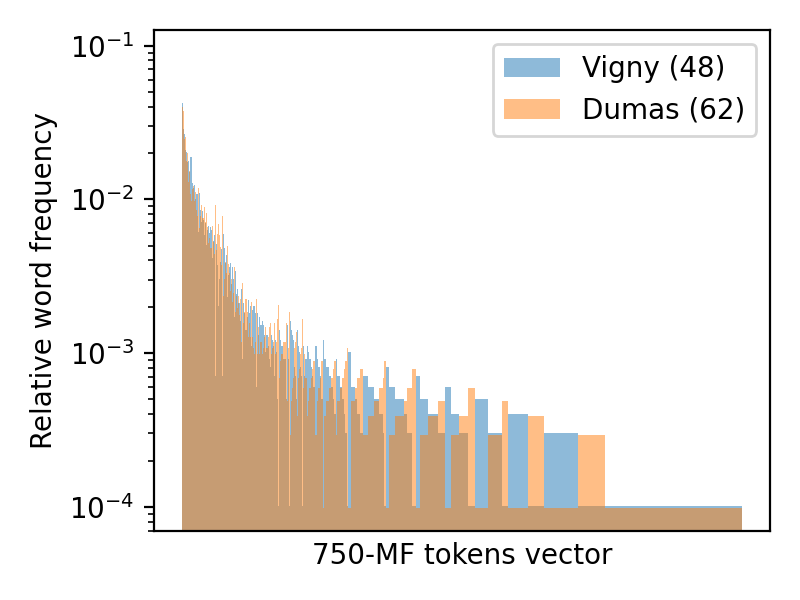
\includegraphics[width=\linewidth]{img/mf_vector_error_0.png}

  \vspace{0.5cm}

  \subcaption{Second example}
  \label{fig:mf_vector_error_1}
  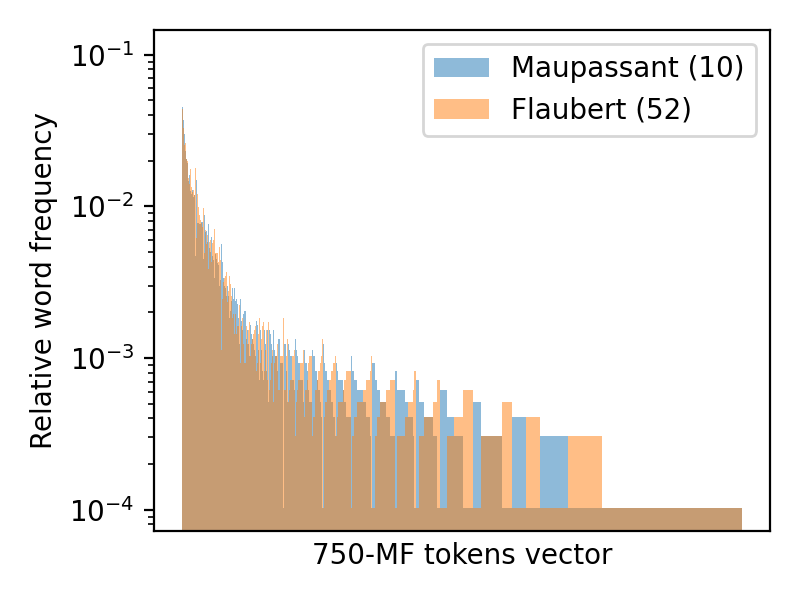
\includegraphics[width=\linewidth]{img/mf_vector_error_1.png}
\end{figure}

\begin{figure}
  \centering
  \caption{750-MF relative frequency for the two documents ranked $X$ in the rank list using the token representation on St-Jean}

  \subcaption{$X$ = First}
  \label{fig:mf_vector_first_rl}
  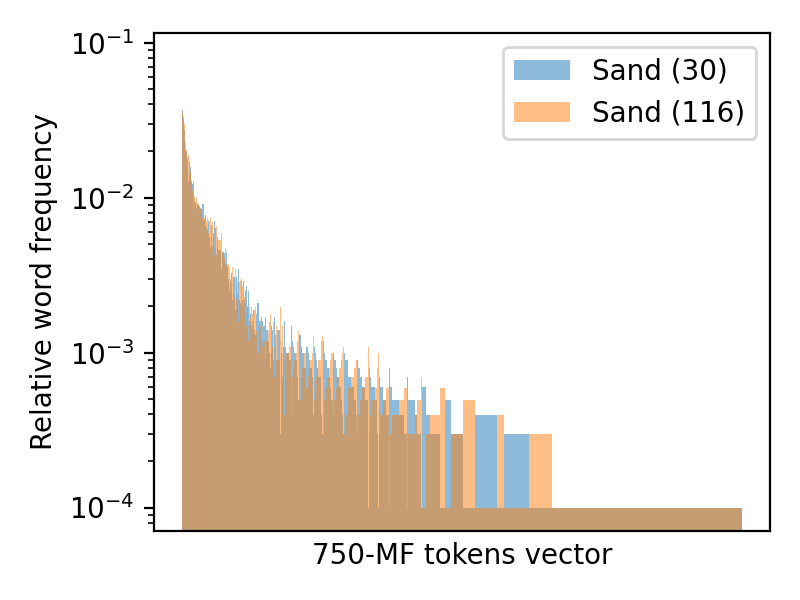
\includegraphics[width=\linewidth]{img/mf_vector_first_rl.png}

  \vspace{0.5cm}

  \subcaption{$X$ = HPrec-th}
  \label{fig:mf_vector_first_last_rl}
  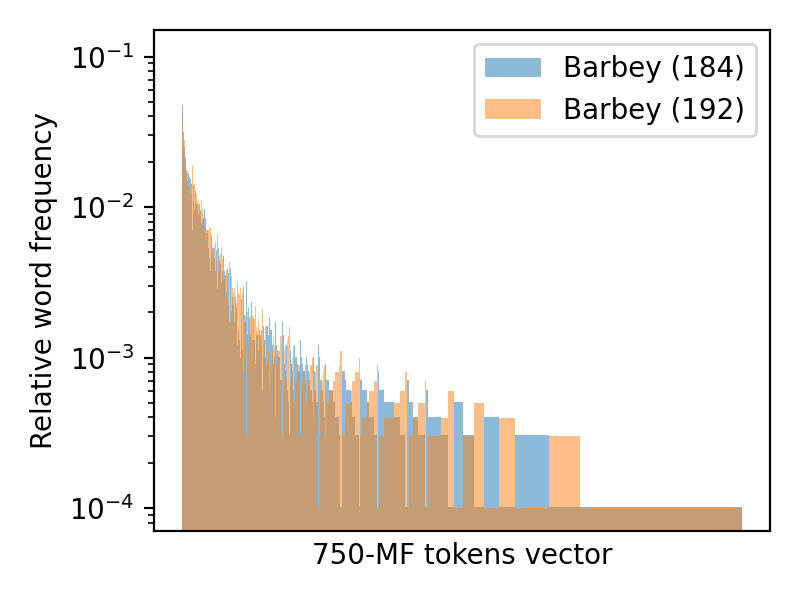
\includegraphics[width=\linewidth]{img/mf_vector_first_last_rl.png}

  \vspace{0.5cm}

  \subcaption{$X$ = Last}
  \label{fig:mf_vector_last_rl}
  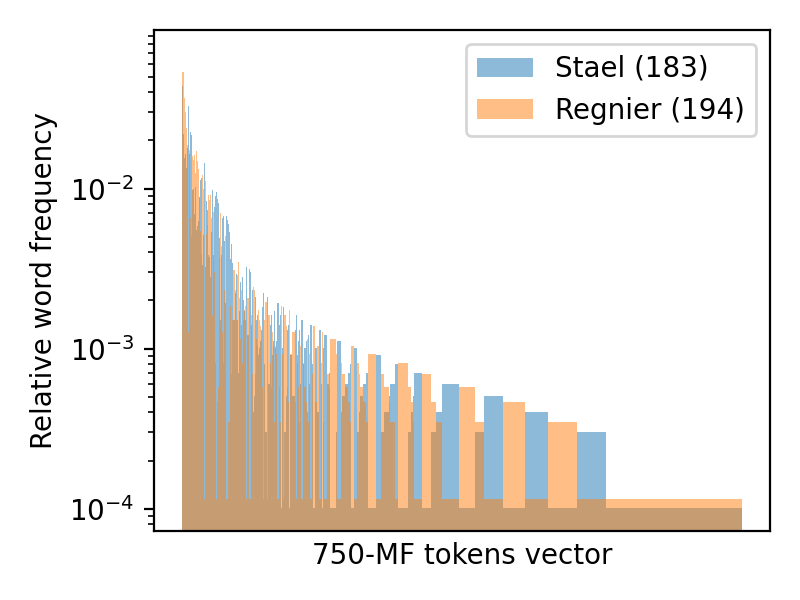
\includegraphics[width=\linewidth]{img/mf_vector_last_rl.png}
\end{figure}
